\documentclass{beamer}
\usepackage{epstopdf}
\usepackage{tabularx}
\usepackage{adjustbox}
\usepackage{pdflscape}
\usepackage[]{hyperref}
\definecolor{links}{HTML}{0B610B} % dark green
%\definecolor{links}{HTML}{2A1B81} % dark blue
\hypersetup{colorlinks,linkcolor=,urlcolor=links}
\usepackage{multirow} % for tables
\usepackage{multicol}
\usepackage{subfig}
\usepackage{graphicx}
\usetheme{Madrid}
\title[Hashing classification for tracking ]{Hashing Classification for charged particle tracking}
\author[Luiza Adelina Ciucu (ATLAS) ]{Luiza Adelina Ciucu (ATLAS)} 

\titlegraphic{
%
\includegraphics[height=2.1cm]{./physics_section_EN_q.eps} 

\includegraphics[height=2.1cm]{./physics_section_EN_q-eps-converted-to.pdf} 
}

\date{19 June 2020}

\begin{document}

\frame{\titlepage}

%\texttt{\detokenize{

% define input folder for our plots only once
\newcommand\inputFolderMergedOld{../backup_01/output_new_ev_000_030}
\newcommand\inputFolderOverlayOld{../backup_01/output_overlay_balanced_ev_000_030}
\newcommand\inputFolderMerged{../output_new_ev_000_100}
\newcommand\inputFolderOverlay{../output_overlay_balanced_ev_000_100}

% add some useful definitions
%\def\MeV{\ifmmode {\mathrm{\ Me\kern -0.1em V}}\else
%                   \textrm{Me\kern -0.1em V}\fi}%  

\def\volumeID{\texttt{\detokenize{volume_id}}}
\def\layerID{\texttt{\detokenize{layer_id}}}

\def\TP{\ifmmode {\mathrm{TP}}\else
                   \textrm{TP}\fi}%
\def\FP{\ifmmode {\mathrm{FP}}\else
                   \textrm{FP}\fi}%                                     
\def\FN{\ifmmode {\mathrm{FN}}\else
                   \textrm{FN}\fi}%
\def\TN{\ifmmode {\mathrm{TN}}\else
                   \textrm{TN}\fi}%

% intro slide
\begin{frame}{Introduction}
\begin{enumerate}
\item[o] Compare 3 methods to balance nb of positive and negative hits: 
\begin{enumerate}
\item[-] A: Unbalanced 30 events. Train 2.29M buckets. Test 0.95 buckets. 
\item[-] B: Balanced 30 events. Train 1.39 M buckets. Test 0.61 buckets. 
\item[-] Not trained: Unbalanced 100 events. Train 7.35 M buckets. Test 3.22. 
\item[-] C: Balanced2 100 events. Train 2.21M buckets. Test 0.98 buckets. 
\end{enumerate}
\item[o] A and C similar nb of buckets, so a fair comparison.
\item[o] For each group of 10: 7 in train, 3 in test. 
\item[o] A=Unbalanced: keep all buckets.
\item[o] B=Balanced: remove buckets (from the left) so that bucket distribution is symmetric around 10 in NbPositiveHit per bucket.
\item[o] C=Balanced2: similar to B, but cut the peak so that same number of buckets between 6-14 inclusive. \\ Also 0,1, 19, 20 are kept as they are. \\ But 2, 3, 4, 5, 15, 16, 17, 18 remain as in B. 
\item[o] Used min 0, 4, 7 and 10 positive hits in the bucket; if less, consider all hits in the bucket to be negative, but use same balancing as above.
\end{enumerate}
\end{frame}
\clearpage



\begin{frame}{Introduction 2}
\begin{enumerate}
\item[o] Reminder how a bucket is created:
\begin{enumerate}
\item[-] Loop over events, and for each event build annoy index and then:
\item[-] Loop over hits and for each hit build a bucket using annoy and 20 nearest neighbours by direction
\item[-] Loop over hits in the bucket, find their particleID; find particleID with most hits in the bucket; denote it majority particle.
\item[-] Loop over hits in the bucket again, if belongs to the majority particle assign output +1, else -1.
\end{enumerate}
\end{enumerate}
\end{frame}
\clearpage

\begin{frame}{Bucket balancing procedure 1/4}
\begin{enumerate}
\item[o] Remove buckets so that bucket distribution is symmetric around 10 in NbPositiveHit per bucket (with default weight of 1.0): Train and Test.
\item[o] Input: \texttt{\detokenize{nparray_output}} (Nx20)
\item[o] Output: \texttt{\detokenize{nparray_outputBalanced}} (Nx20)
\item[o] Step 1: count buckets for each category of nbPositiveHit
\begin{enumerate}
\item[-] output: \texttt{\detokenize{dict_nbPositiveHit_counterBucket}}
\item[-] process: loop over buckets, for each bucket count positive hits into nbPositiveHit, increase counter in dicti at that key of nbPositiveHit.
\end{enumerate}
\item[o] The result is shown below for Train. Note not balanced around 10. 
\end{enumerate}
\centering
% plots
\includegraphics[width=0.5\textheight]{\inputFolderMergedOld/CounterUnbalanced.png}
\end{frame}

\begin{frame}{Bucket balancing procedure 2/4}
\begin{enumerate}
\item[o] Step 2: from this (unbalanced) dict calculate desired balanced dict. 
\begin{enumerate}
\item[-] input: \texttt{\detokenize{dict_nbPositiveHit_counterBucket}}
\item[-] output: \texttt{\detokenize{dict_nbPositiveHit_counterBucket_Balanced}}
\item[-] process: loop over i from the first half of nbPositiveHit (from 0 to 10)
\item[-] nbLeft=\texttt{\detokenize{dict_nbPositiveHit_counterBucket[i]}}
\item[-] nbRight=\texttt{\detokenize{dict_nbPositiveHit_counterBucket[20-i]}}
\item[-] Find nbMin from nbLeft and nbRight
\item[-] Set in the new balanced dictionary both values ot the nbMin
\item[-] \texttt{\detokenize{dict_nbPositiveHit_counterBucke_Balancedt[i]=nbMin}}
\item[-]\texttt{\detokenize{dict_nbPositiveHit_counterBucke_Balancedt[20-i]=nbMin}}
\end{enumerate}
\item[o] The result is shown below for Train. Note it is balanced around 10. 
\item[o] Right usually smaller, so remains the same and remove from left.
\item[o] nbPositiveHit 0 and 1 have counts of 0, $\rightarrow$ set 19 and 20 to zero.
\end{enumerate}
\centering
% plots
\includegraphics[width=0.32\textheight]{\inputFolderMergedOld/CounterUnbalanced.png}
\end{frame}

\begin{frame}{Bucket balancing procedure 3/4}
\begin{enumerate}
\item[o] Step 3: use desired balanced dict to obtain balanced output.
\begin{enumerate}
\item[-] input: \texttt{\detokenize{dict_nbPositiveHit_counterBucket_Balanced}}
\item[-] input: \texttt{\detokenize{nparray_output}} (Nx20)
\item[-] output: \texttt{\detokenize{nparray_outputBalanced}} (Nx20)
\item[-] process: loop over buckets from \texttt{\detokenize{nparray_output}}:
\item[-] find nbPositiveHit for the bucket
\item[-] from nbPositiveHit find desired number of bucket in this category
\item[-] count the current number of buckets in this category
\item[-] if current counter $\le$ desired number, append to a list
\item[-] else (do nothing, so skip it)
\item[-] .
\item[-] after for loop convert list to \texttt{\detokenize{nparray_outputBalanced}}
\item[-] as in step 1, calculate dictionary of counterBucket for each category
\item[-] by printing verify it is the same as the one desired (confirmed)
\item[-] next overlay histograms for nbPositiveHit in Unbalanced and Balanced
\item[-] as expected, now it is balanced, the right side is the same in both cases, and we removed buckets from the left
\item[-] But we set 19 and 20 to zero, to keep as 0 and 1. Though 0 will always have no buckets. But otherwise makes the symmetry harder.
\end{enumerate}
\end{enumerate}
\end{frame}



\begin{frame}{Bucket balancing method 2}
\begin{enumerate}
\item[o] Similar to Balanced from before (above), but with some changes.
\item[o] Cut the peak so that same number of buckets between 6-14 inclusive.
\item[o] Also 0,1, 19, 20 are kept as they are. 
\begin{enumerate}
\item[-] No buckets with nbPositiveHit=0, so it is unfair to set nbPositiveHit=20 to zero as well.
\item[-] Only 3 nbPositiveHit=3, so it is unfair to set nbPositiveHit=19 to 3.
\end{enumerate}
\item[o] But 2, 3, 4, 5, 15, 16, 17, 18 remain as in B. 
\end{enumerate}
\centering
% plots
\includegraphics[height=0.4\textheight]{\inputFolderMerged/Balanced2.png}
\end{frame}



\begin{frame}{Histogram NbBuckets vs NbPositiveHit in a bucket.}
\begin{enumerate}
\item[o] 30 events. \textcolor{red}{Unbalanced} (\textcolor{blue}{Balanced})  \textcolor{red}{are not} (\textcolor{blue}{are}) symmetric around 10. 
\end{enumerate}
\centering
% plots
\includegraphics[width=0.48\textwidth]{\inputFolderMergedOld/plot_histo_2_NbBucket_vs_NbPositiveHit_Train.pdf}
\includegraphics[width=0.48\textwidth]{\inputFolderMergedOld/plot_histo_2_NbBucket_vs_NbPositiveHit_Test.pdf}\\
\includegraphics[width=0.48\textwidth]{\inputFolderMergedOld/plot_histo_2_NbBucket_vs_NbPositiveHit_normalized_Train.pdf}
\includegraphics[width=0.48\textwidth]{\inputFolderMergedOld/plot_histo_2_NbBucket_vs_NbPositiveHit_normalized_Test.pdf}\\
\end{frame}

\begin{frame}{Histogram NbBuckets vs NbPositiveHit in a bucket.}
\begin{enumerate}
\item[o] 100 events. \textcolor{red}{Unbalanced} vs \textcolor{blue}{Balanced2}.
\end{enumerate}
\centering
% plots
\includegraphics[width=0.48\textwidth]{\inputFolderMerged/plot_histo_2_NbBucket_vs_NbPositiveHit_Train.pdf}
\includegraphics[width=0.48\textwidth]{\inputFolderMerged/plot_histo_2_NbBucket_vs_NbPositiveHit_Test.pdf}\\
\includegraphics[width=0.48\textwidth]{\inputFolderMerged/plot_histo_2_NbBucket_vs_NbPositiveHit_normalized_Train.pdf}
\includegraphics[width=0.48\textwidth]{\inputFolderMerged/plot_histo_2_NbBucket_vs_NbPositiveHit_normalized_Test.pdf}\\
\end{frame}



%\begin{frame}{Count buckets in each NbPositiveHit category.}
%\begin{enumerate}
%\item[o] Balanced around 10 NbPositiveHit via bucket removal.
%\item[o] 0 and 1 no buckets $\rightarrow$ 19 and 20 are balanced to no buckets (ignored). 
%\end{enumerate}
%\centering
% plots
%\includegraphics[width=0.8\textheight]{\inputFolderMergedOld/Balanced_30_buckets.png}
%\end{frame}



\begin{frame}{OutputPositive and PredictedOutputPositive 1/2}
\begin{enumerate}
\item[o] Min00 (left) and Min04 (right)
\end{enumerate}
\centering
% plots
\includegraphics[width=0.43\textwidth]{\inputFolderOverlay_Min00/plot_02_1_overlay_histo_OutputPositive_Test.pdf}
\includegraphics[width=0.43\textwidth]{\inputFolderOverlay_Min04/plot_02_1_overlay_histo_OutputPositive_Test.pdf}\\
\includegraphics[width=0.43\textwidth]{\inputFolderOverlay_Min00/plot_02_1_overlay_histo_PredictedOutputPositive_Test.pdf}
\includegraphics[width=0.43\textwidth]{\inputFolderOverlay_Min04/plot_02_1_overlay_histo_PredictedOutputPositive_Test.pdf}\\
\end{frame}

\begin{frame}{OutputPositive and PredictedOutputPositive 2/2}
\begin{enumerate}
\item[o] Min07 (left) and Min10 (right).
\item[o] Min10 and method Unbalanced predicts all hits to be negative.
\end{enumerate}
\centering
% plots
\includegraphics[width=0.43\textwidth]{\inputFolderOverlay_Min07/plot_02_1_overlay_histo_OutputPositive_Test.pdf}
\includegraphics[width=0.43\textwidth]{\inputFolderOverlay_Min10/plot_02_1_overlay_histo_OutputPositive_Test.pdf}\\
\includegraphics[width=0.43\textwidth]{\inputFolderOverlay_Min07/plot_02_1_overlay_histo_PredictedOutputPositive_Test.pdf}
\includegraphics[width=0.43\textwidth]{\inputFolderOverlay_Min10/plot_02_1_overlay_histo_PredictedOutputPositive_Test.pdf}\\
\end{frame}

\begin{frame}{Metrics for each VolumeID overlay two methods 1/2.}
\begin{enumerate}
\item[o] Min00 and Min04 very similar. 
\end{enumerate}
\centering
% table
\begin{center}
\begin{tabular}{ |c|c|c| } 
\hline
Accuracy & Precision & Recall \\ 
\hline
$\frac{\TP+\TN}{\TP+\FP+\FN+\TN}$ & $\frac{\TP}{\TP+\FP}$  & $\frac{\TP}{\TP+\FN}$ \\ 
\hline
\end{tabular}
\end{center}
% plots
\includegraphics[width=0.32\textwidth]{\inputFolderOverlay_Min00/plot_03_1_overlay_graph_Accuracy_VolumeID_Test.pdf}
\includegraphics[width=0.32\textwidth]{\inputFolderOverlay_Min00/plot_03_1_overlay_graph_Precision_VolumeID_Test.pdf}
\includegraphics[width=0.32\textwidth]{\inputFolderOverlay_Min00/plot_03_1_overlay_graph_Recall_VolumeID_Test.pdf}\\
\includegraphics[width=0.32\textwidth]{\inputFolderOverlay_Min04/plot_03_1_overlay_graph_Accuracy_VolumeID_Test.pdf}
\includegraphics[width=0.32\textwidth]{\inputFolderOverlay_Min04/plot_03_1_overlay_graph_Precision_VolumeID_Test.pdf}
\includegraphics[width=0.32\textwidth]{\inputFolderOverlay_Min04/plot_03_1_overlay_graph_Recall_VolumeID_Test.pdf}\\
\end{frame}

\begin{frame}{Metrics for each VolumeID overlay two methods 2/2.}
\begin{enumerate}
\item[o] \item[o] Min10 learns all hits to be negative, so precision and recall at zero.
\end{enumerate}
\centering
% table
\begin{center}
\begin{tabular}{ |c|c|c| } 
\hline
Accuracy & Precision & Recall \\ 
\hline
$\frac{\TP+\TN}{\TP+\FP+\FN+\TN}$ & $\frac{\TP}{\TP+\FP}$  & $\frac{\TP}{\TP+\FN}$ \\ 
\hline
\end{tabular}
\end{center}
% plots
\includegraphics[width=0.32\textwidth]{\inputFolderOverlay_Min07/plot_03_1_overlay_graph_Accuracy_VolumeID_Test.pdf}
\includegraphics[width=0.32\textwidth]{\inputFolderOverlay_Min07/plot_03_1_overlay_graph_Precision_VolumeID_Test.pdf}
\includegraphics[width=0.32\textwidth]{\inputFolderOverlay_Min07/plot_03_1_overlay_graph_Recall_VolumeID_Test.pdf}\\
\includegraphics[width=0.32\textwidth]{\inputFolderOverlay_Min10/plot_03_1_overlay_graph_Accuracy_VolumeID_Test.pdf}
\includegraphics[width=0.32\textwidth]{\inputFolderOverlay_Min10/plot_03_1_overlay_graph_Precision_VolumeID_Test.pdf}
\includegraphics[width=0.32\textwidth]{\inputFolderOverlay_Min10/plot_03_1_overlay_graph_Recall_VolumeID_Test.pdf}\\
\end{frame}




\begin{frame}{Metrics for each VolumeID with min value used.}
\begin{enumerate}
\item[o] Min00 and Min04 very similar. 
\item[o] Min10 learns all hits to be negative, so precision and recall at zero.
\end{enumerate}
\centering
% plots
\includegraphics[width=0.28\textwidth]{\inputFolderOverlayOld_Unbalanced/plot_03_1_overlay_graph_Accuracy_VolumeID_Test.pdf}
\includegraphics[width=0.28\textwidth]{\inputFolderOverlayOld_Unbalanced/plot_03_1_overlay_graph_Precision_VolumeID_Test.pdf}
\includegraphics[width=0.28\textwidth]{\inputFolderOverlayOld_Unbalanced/plot_03_1_overlay_graph_Recall_VolumeID_Test.pdf}\\
\includegraphics[width=0.28\textwidth]{\inputFolderOverlayOld_Balanced/plot_03_1_overlay_graph_Accuracy_VolumeID_Test.pdf}
\includegraphics[width=0.28\textwidth]{\inputFolderOverlayOld_Balanced/plot_03_1_overlay_graph_Precision_VolumeID_Test.pdf}
\includegraphics[width=0.28\textwidth]{\inputFolderOverlayOld_Balanced/plot_03_1_overlay_graph_Recall_VolumeID_Test.pdf}\\
\includegraphics[width=0.28\textwidth]{\inputFolderOverlay_Balanced/plot_03_1_overlay_graph_Accuracy_VolumeID_Test.pdf}
\includegraphics[width=0.28\textwidth]{\inputFolderOverlay_Balanced/plot_03_1_overlay_graph_Precision_VolumeID_Test.pdf}
\includegraphics[width=0.28\textwidth]{\inputFolderOverlay_Balanced/plot_03_1_overlay_graph_Recall_VolumeID_Test.pdf}\\
\end{frame}



\begin{frame}{Conclusion. Future plans.}
\begin{enumerate}
\item[o] Conclusions:
  \begin{enumerate}
\item[-] Compared 3 methods: Unbalanced vs Balanced vs Balanced2.
\item[-] Balanced: remove buckets such that number of buckets with a given nbPositiveHit is symmetric around 10.
\item[-] Balanced2: Same as Balanced, but reduce peak to have a flatter distribution (same values between 6-14), keep also 19 and 20 to non-zero.
\item[-] Min00 and Min04 are very similar.
\item[-] Min07 in between Min04 and Min10.
\item[-] Overall, balancing buckets improve performance.
\item[-]  \textbf{Could choose 100 events, Balanced2, with Min04.}
\end{enumerate}
\item[o] Future plans:
\begin{enumerate}
\item[-] Balance buckets in the $\eta$ of the majority-particle.
\item[-] Write master thesis.
\end{enumerate}
\end{enumerate}
\end{frame}

\end{document}

\begin{frame}{Conclusion. Future plans.}
\begin{enumerate}
\item[o] Conclusions:
\begin{enumerate}
\item[-] Compared two methods: Unbalanced vs Balanced.
\item[-]
\item[-]
\end{enumerate}
\item[o] Future plans:
\begin{enumerate}
\item[-]
\item[-]
\item[-]
\end{enumerate}
\end{enumerate}
\end{frame}

\end{document}

% intro slide
\begin{frame}{Introduction}
\begin{enumerate}
\item[o] Compare two methods to balance the number of positive and negative hits : unbalanced (A) and balanced (B).
\item[o] Used 30 events. Each group of 10: 7 in train, 3 in test. 
\item[o] Unbalanced (A): keep all buckets (with default weight of 1.0).
\item[o] Balanced (B): remove buckets so that bucket distribution is symmetric around 10 in NbPositiveHit per bucket (with default weight of 1.0).
\item[o] Used min 0, 4, 7 and 10 positive hits in the bucket; if less, consider all hits in the bucket to be negative, but use same reweighting as above.
\item[o] How a bucket is created:
\begin{enumerate}
\item[-] Loop over events, and for each event build annoy index and then:
\item[-] Loop over hits and for each hit build a bucket using annoy and 20 nearest neighbours by direction
\item[-] Loop over hits in the bucket, find their particleID; find particleID with most hits in the bucket; denote it majority particle.
\item[-] Loop over hits in the bucket again, if belongs to the majority particle assign output +1, else -1.
\end{enumerate}
\end{enumerate}
\end{frame}
\clearpage